The previously discussed demand for high-resolution simulation with optimal
performance and robustness motivated the development of our novel co-rotational
elasticity discretization. Following \cite{Chao:2010:SGM}, we use an accurate
treatment of force derivatives to yield a more robust solver than the
simplified warped-stiffness techniques. We show that these careful
linearizations can be done both cheaply and simply and are essential for our desired
robustness and efficiency. We perform our discretization over a
uniform hexahedral lattice  (rather than an unstructured tetrahedral one) to
facilitate performance on modern hardware. Although standard methods for
hexahedra require 8 point Gauss quadrature per cell for stability, we develop a
much more efficient one-point quadrature discretization
(section~\ref{sec:stabilization}).

\subsection{Fundamentals}
\label{sec:fundamentals}

We represent the deformation of a 3D elastic body by a function $\vec{\phi}:\Omega\rightarrow\mathbf{R}^3$, which maps a material point
$\vec{X}$ to a deformed world-space point $\vec{x}$ so $\vec{x}=\vec{\phi}(\vec{X})$. Subsequently, we use $\vec{x}$ and $\vec{\phi}$ interchangeably,
i.e.\ we identify $\vec{x}(\vec{X})\equiv\vec{\phi}(\vec{X})$. For hyperelastic
materials in general, the response can be computed based on the deformation energy:
\begin{equation}
E=\int_\Omega\Psi(\vec{X},\mathbf{F}(\vec{X}))d\vec{X}
\label{eqn_energy_integral}
\end{equation}
For simplicity we will here consider the energy density $\Psi$ as a function of the
deformation gradient $F_{ij}=\partial\phi_i/\partial\vec{X}_j$. Specifically for
corotational elasticity we have
%For typical materials, the elastic energy density $\Psi$ appearing in equation (\ref{eqn_energy_integral}) is a function of the Jacobian of $\phi$, also known as the  deformation gradient  
%$\mathbf{F}$ (i.e.\ $F_{ij}=\partial\phi_i/\partial\vec{X}_j$). The additional explicit dependence of $\mathbf{F}$ on the material coordinates $\vec{X}$ allows for inhomogeneous material
%parameters; for simplicity we shall initially focus on homogeneous elasticity where $\Psi$ is purely a function of $\mathbf{F}$. Corotational linear elasticity defines this energy
%density as follows:
\begin{equation}
\Psi=\mu\|\mathbf{F}-\mathbf{R}\|_F^2+\frac{\lambda}{2}\tr^2(\mathbf{R}^T\mathbf{F}-\mathbf{I})
\label{eqn_energy_F}
\end{equation}
where $\mu,\lambda$ are the Lam\'{e} coefficients, and $\mathbf{R}$ is the rotation from the polar decomposition $\mathbf{F}=\mathbf{RS}$.

\subsection{Energy discretization}

We discretize our model domain $\Omega$ into cubic elements $\Omega_e$ of step size $h$ so $\Omega=\cup_e\Omega_e$. The degrees of freedom are world space samples of
$\vec{x}_i=\vec{\phi}(\vec{X}_i)$. The discrete version of
equation~(\ref{eqn_energy_integral}) then becomes a sum of energies from each element $E_e$.  Using just a single quadrature point for the voxel center $\vec{p}^c$ gives $E_e \approx h^3\Psi(\mathbf{F}^e)$ where $\mathbf{F}^e\approx\mathbf{F(\vec{p}^c)}$ is computed with central differences about the cell center from averaged faces.
\begin{figure}
\centering
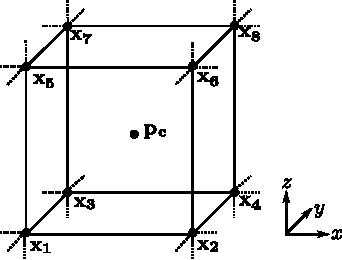
\includegraphics[width=.35\columnwidth]{elasticity/figures/grid.pdf}
\caption{A sample cubic element.}\label{fig:cubic_element}
\end{figure}
 This approximation can be written
\begin{equation}
F_{ij}^e=\sum_kG_{jk}^ex_k^{(i)}
\label{eqn_discrete_gradient}
\end{equation}
where $x_k^{(i)}$ is the $i$-th component of the three-dimensional vector $\vec{x}_k$ (see Figure~\ref{fig:cubic_element}) and we have
a \emph{discrete gradient}
{\small$$
\mathbf{G}^e=
\frac{1}{4h}
\left(
\begin{array}{cccccccc}
-1 &  1 & -1 &  1 & -1 &  1 & -1 &  1 \\
-1 & -1 &  1 &  1 & -1 & -1 &  1 &  1 \\
-1 & -1 & -1 & -1 &  1 &  1 &  1 &  1
\end{array}
\right).
$$}
Finally, we have a means to compute the total energy in terms only of the nodal world positions of our hexahedral lattice.



\begin{figure}[th]
\center{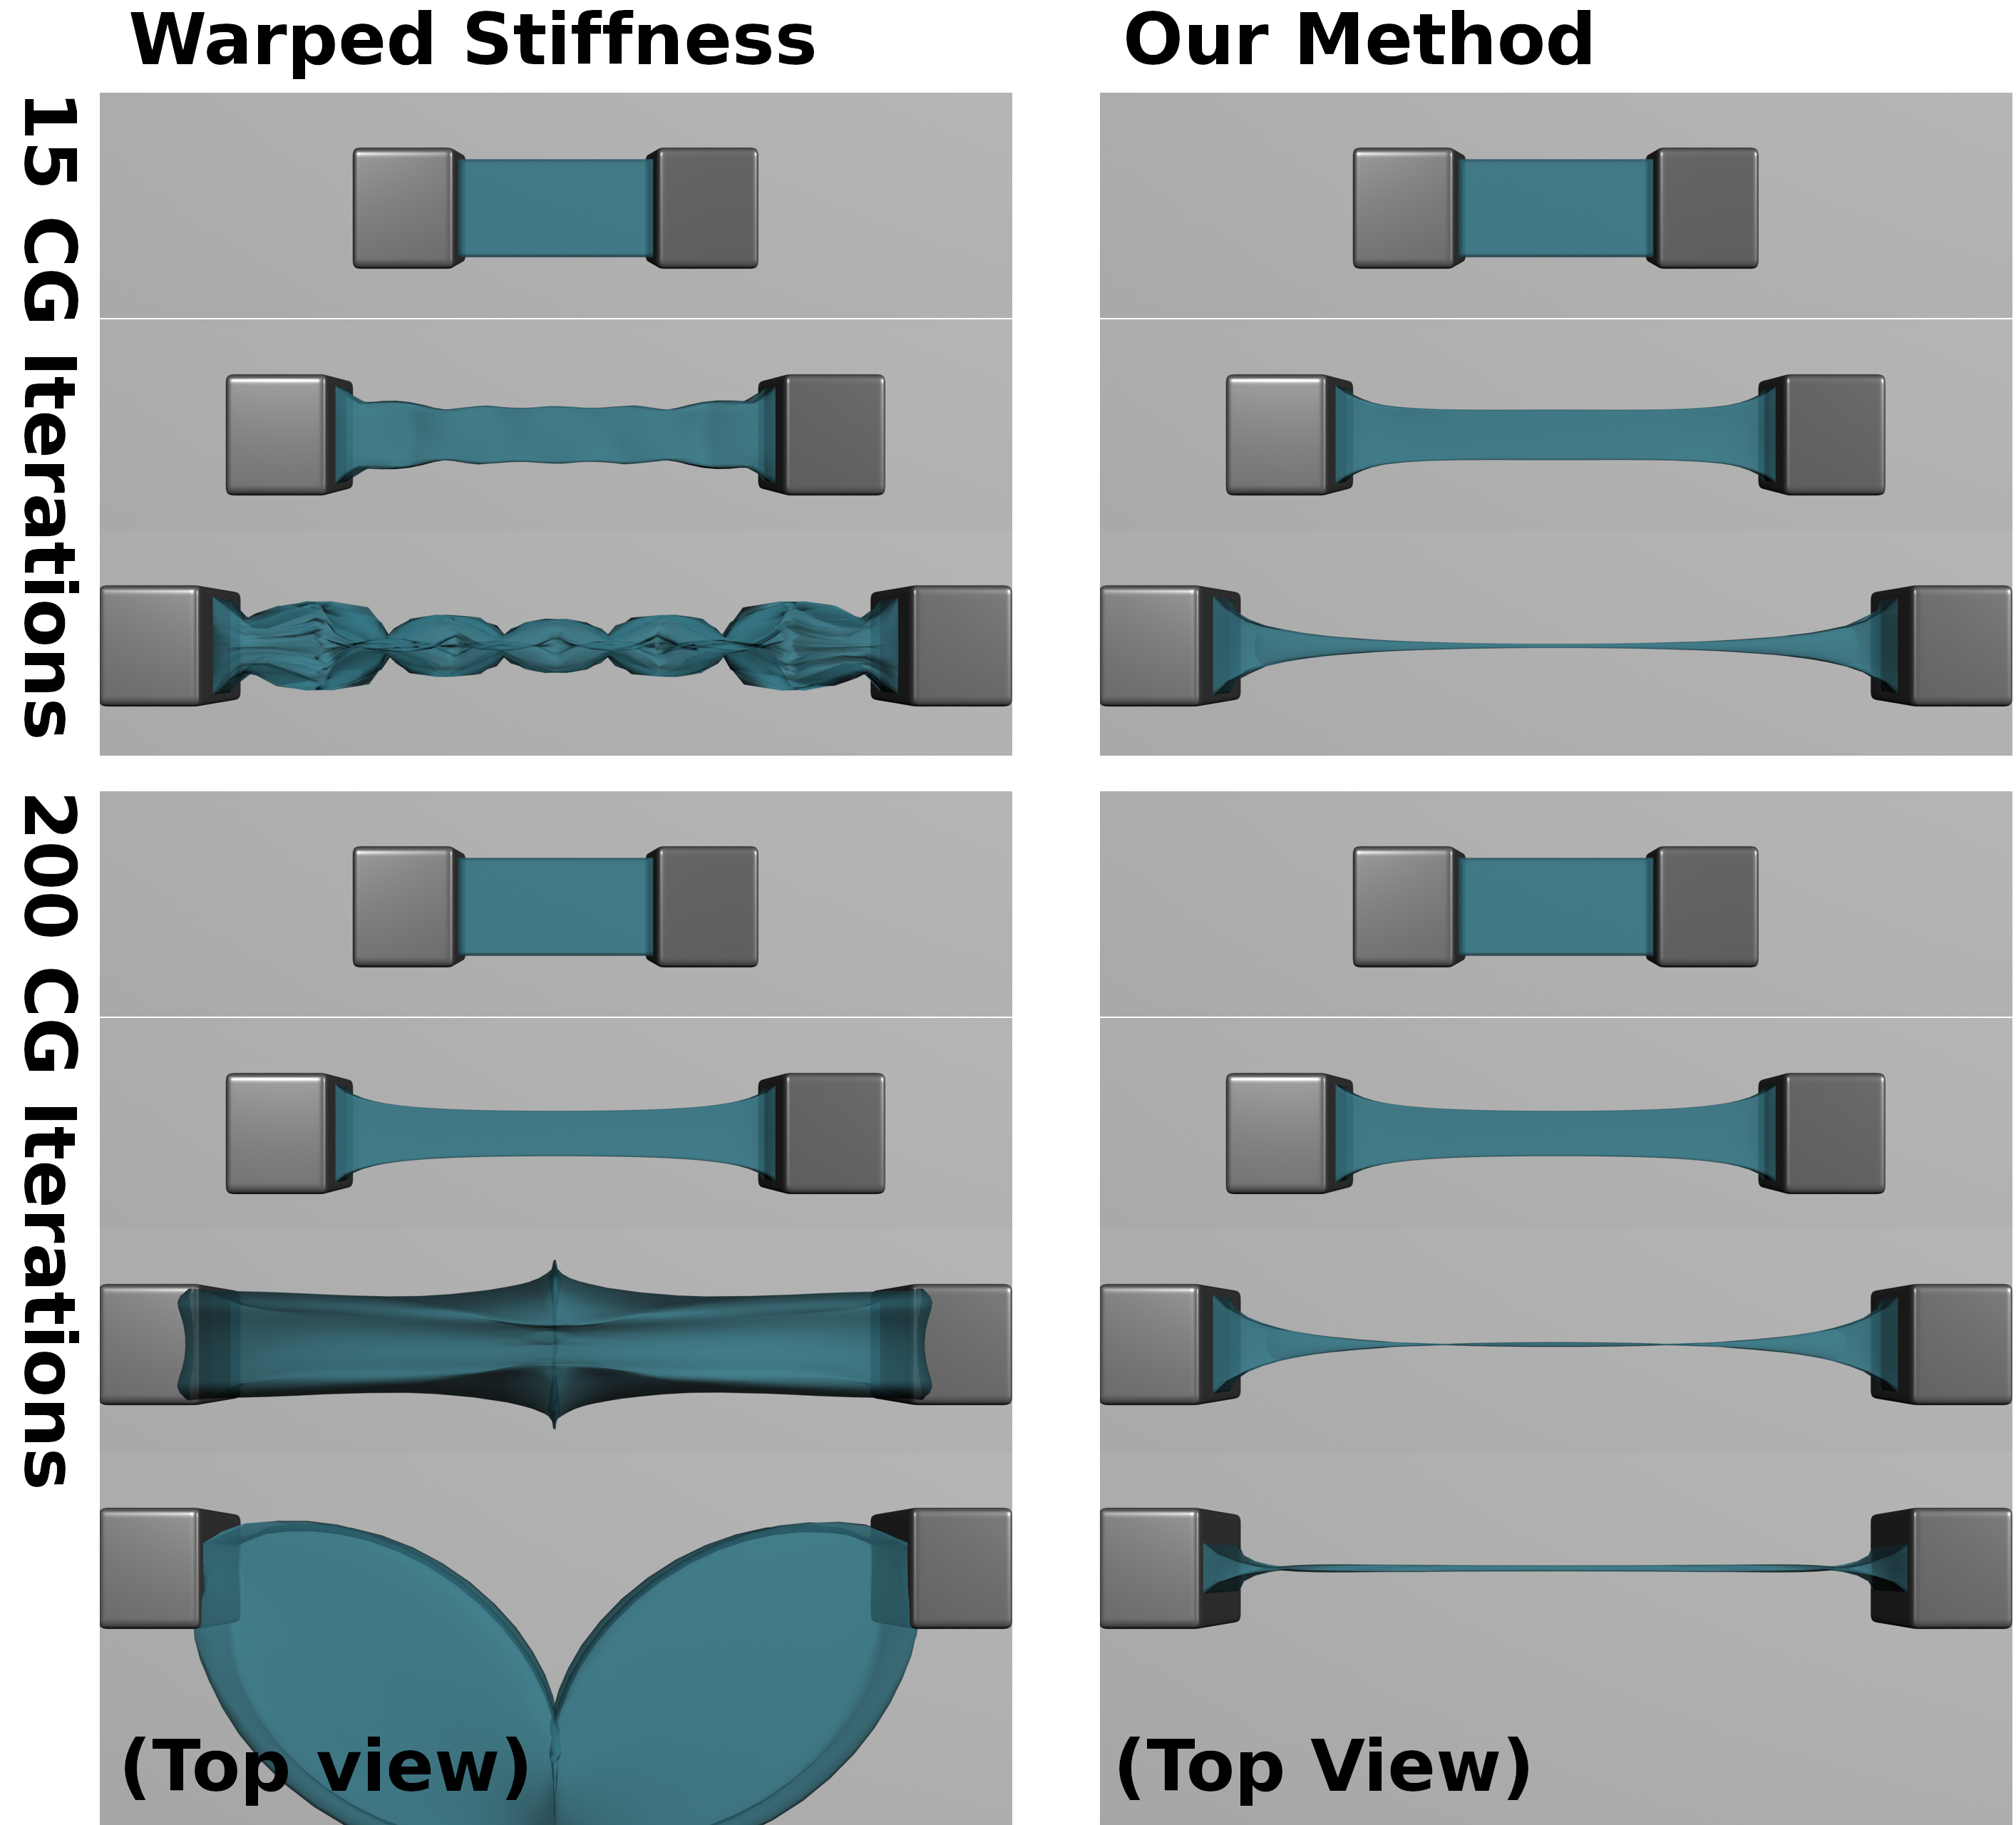
\includegraphics[width=.7\linewidth]{elasticity/figures/warpedcomp}}
\caption{Inexact methods of computing force differentials lead to instabilities
unlike our method}
\label{fig:warpedstiff}
\end{figure}

\subsection{Force and equilibrium}
\label{sec:force}

A discrete force per node can in general be written as
\begin{equation}
\vec{f}_i=-\frac{\partial E}{\partial\vec{x}_i}=\sum_e\left(-\frac{\partial E_e}{\partial\vec{x}_i}\right)=\sum_e\vec{f}_i^e.
\label{eqn_elemental_forces}
\end{equation}
%Intuitively, we identify the quantity $\vec{f}_i^e=-\partial E_e/\partial\vec{x}_i$ in the last equation with the contribution of element $\Omega_e$ to the forces exerted on node
%$\vec{x}_i$.
 Using equation (\ref{eqn_discrete_gradient}) and the fact that $\Psi$ is a function of the deformation gradient alone, a concise expression for each of the components
of $\vec{f}_i^e=(f_i^{(1)},f_i^{(2)},f_i^{(3)})$ (the force contribution to node $i$ from element $e$) is: 
\begin{eqnarray}
f_i^{(j)}\!\!\!&\!\!\!=\!\!\!&\!\!\!-\frac{\partial E_e}{\partial\vec{x}_i^{(j)}}=-V_e\frac{\partial\Psi(\mathbf{F}^e)}{\partial\vec{x}_i^{(j)}}
=
-V_e\sum_{k,l}\left.\frac{\partial\Psi}{\partial F_{kl}}\right|_{\mathbf{F}^e}\frac{\partial F_{kl}^e}{\partial\vec{x}_i^{(j)}} \nonumber \\
\!\!\!&\!\!\!=\!\!\!&\!\!\!
-V_e\sum_{k,l}[\mathbf{P}(\mathbf{F}^e)]_{kl}G_{li}^e\delta_{jk}
=
-V_e\sum_l[\mathbf{P}(\mathbf{F}^e)]_{jl}G_{li}^e \nonumber \\
\!\!\!&\!\!\!=\!\!\!&\!\!\!
-V_e[\mathbf{P}(\mathbf{F}^e)\mathbf{G}^e]_{ji}.
\label{eqn_nodal_forces}
\end{eqnarray}
where $\mathbf{P}(\mathbf{F})\!:=\!\partial\Psi/\partial\mathbf{F}$ is
the 1st Piola-Kirchhoff stress tensor.

To compute $\mathbf{P}(\mathbf{F})$ for corotational elasticity from
Equation~(\ref{eqn_energy_F}), we begin by noting that the matrix $\delta\mathbf{R}^T\mathbf{R}$
is skew symmetric.  This can be shown by taking differentials of
$\mathbf{R}^T\mathbf{R}=\mathbf{I}$ to get $\mathbf{R}^T\!\delta\mathbf{R})^T+\mathbf{R}^T\!\delta\mathbf{R}=0$.
Consequently 
\begin{align}
\tr(\delta\mathbf{R}^T\mathbf{F})&=\tr(\delta\mathbf{R}^T\mathbf{RS})\nonumber\\
        &=(\delta\mathbf{R}^T\mathbf{R}):\mathbf{S}\nonumber\\
        &=0\label{eqn:tr_dRt_F}
\end{align} 
as a contraction of a
symmetric and a skew symmetric matrix. 

Taking differentials of the energy density in
equation~(\ref{eqn_energy_F}), we compute
\begin{align*}
\delta\mathbf{\Psi} =&
2\mu(\mathbf{F}-\mathbf{R}):\delta\mathbf{F}-2\mu(\mathbf{F}-\mathbf{R}):\delta\mathbf{R}\\
&+\lambda\tr(\mathbf{R}^T\mathbf{F}-\mathbf{I})\left(\tr(\mathbf{R}^T\delta\mathbf{F})+\tr(\delta\mathbf{R}^T\mathbf{F})\right)\\
=&2\mu(\mathbf{F}-\mathbf{R}):\delta\mathbf{F}-2\mu\tr(\delta\mathbf{R}^T\mathbf{F})-2\mu\tr(\delta\mathbf{R}^T\mathbf{R})\\
 &+\lambda\tr(\mathbf{R}^T\mathbf{F}-\mathbf{I})\left(\mathbf{R}:\delta\mathbf{F}+\tr(\delta\mathbf{R}^T\mathbf{F})\right)
\end{align*}
Using the skew-symmetry of $\delta\mathbf{R}^T\mathbf{R}$
and equation~(\ref{eqn:tr_dRt_F}), we can eliminate all
$\delta\mathbf{R}$ terms to get
\begin{equation}
\delta\Psi=\left(2\mu(\mathbf{F}-\mathbf{R})+\lambda\tr(\mathbf{R}^T\mathbf{F}-\mathbf{I})\mathbf{R}\right):\delta\mathbf{F}.\label{eqn:dPsi}
\end{equation}
Since $\delta\Psi = \partial\Psi/\partial\mathbf{F}:\delta\mathbf{F} = \mathbf{P}:\delta\mathbf{F}$, we can compute 
\begin{align}
\mathbf{P}&=2\mu\left(\mathbf{F}-\mathbf{R}\right) + \lambda \tr(\mathbf{R}^T\mathbf{F}-\mathbf{I})\mathbf{R}\nonumber\\
        &=\mathbf{R}\left[2\mu(\mathbf{S}-\mathbf{I})+\lambda \tr(\mathbf{S}-\mathbf{I})\right].\label{eqn_piola_stress}
\end{align}


Combining this with equation~\ref{eqn_nodal_forces} we have a matrix
that maps the nodal positions of a cell to its force contribution
\begin{equation}
\mathbf{J}^e
=
\left(
\begin{array}{cccc}
\vec{f}_1^e &
\vec{f}_2^e &
\cdots &
\vec{f}_8^e
\end{array}
\right)
=-V_e\mathbf{P}(\mathbf{F}^e)\mathbf{G}^e.
\label{eqn_cell_forces}
\end{equation}

At each nodal position $\vec{x}:=(\vec{x}_1,\ldots,\vec{x}_N)$ we compute the
forces $\vec{f}(\vec{x}):=(\vec{f}_1(\vec{x}_1),\ldots,\vec{f}_N(\vec{x}_N))$
and we might additionally have external forces $\mathbf{g}$. We solve
the resulting force balance equation $\mathbf{f}+\mathbf{g}=0$ using
Newton-Raphson where the $k$th iterate requires the solution of the linearized
system:
\begin{equation}
\mathbf{K}(\vec{x}^{(k)})\delta\vec{x}^{(k)}=\vec{g}+\vec{f}(\vec{x}^{(k)}).
\label{eqn_newton_step}
\end{equation}
$
\mbox{Here}\ \ 
\mathbf{K}(\vec{x}^{(k)}):=-\left.\frac{\partial\vec{f}}{\partial\vec{x}}\right|_{\vec{x}^{(k)}}
\ \ \mbox{and}\ \ 
\delta\vec{x}^{(k)}:=\vec{x}^{(k+1)}\!-\!\vec{x}^{(k)}
$.

\subsection{Differentials of force and stress}


Equation~(\ref{eqn_newton_step}) requires solving $\mathbf{K}$ at every
iteration. However, forming the matrix explicitly would incur significant performance losses from the 243 non-zero entries needed per node. Instead, we define a procedure that directly
determines the product $\mathbf{K}\delta\vec{x}$ (where $\delta\vec{x}$ is a
displacement), allowing the use of a Krylov solver. The product
$\mathbf{K}\delta\vec{x}\!=\!-\delta\vec{f}$ is the force differential induced
by the displacements.


%with an input vector $\delta\vec{x}$ without requiring $\mathbf{K}$ to be
%explicitly formed. Such a routine will be sufficient for a Krylov solver for equation (\ref{eqn_newton_step}), or for the multigrid approach proposed in section \ref{sec:multigrid}.

Applying differentials on equations (\ref{eqn_elemental_forces}) and (\ref{eqn_cell_forces}) we can write the differential of each nodal force
as $\delta\vec{f}_i\!=\!\sum_e\delta\vec{f}_i^e$, where:
\begin{equation}
\left(
\begin{array}{cccc}
\delta\vec{f}_1^e &
\delta\vec{f}_2^e &
\cdots &
\delta\vec{f}_8^e
\end{array}
\right)
=-h^3\delta\left[\mathbf{P}(\mathbf{F}^e)\right]\mathbf{G}^e.
\label{eqn_elemental_force_differentials}
\end{equation}

Taking differentials on equation (\ref{eqn_piola_stress}) and using
equation (\ref{eqn:tr_dRt_F}), we obtain
\begin{align}
  \delta\mathbf{P}=&2\mu(\delta\mathbf{F}-\delta\mathbf{R})+\lambda\left[\tr(\delta\mathbf{R}^T\mathbf{F})
  +\tr(\mathbf{R}^T\delta\mathbf{F})\right]\mathbf{R}\nonumber \\ 
  &+\lambda\tr(\mathbf{R}^T\mathbf{F}-\mathbf{I})\delta\mathbf{R} \nonumber \\
  =&2\mu\delta\mathbf{F}+\lambda\tr(\mathbf{R}^T\delta\mathbf{F})\mathbf{R}
  +\left[\lambda\tr(\mathbf{S}-\mathbf{I})-2\mu\right]\delta\mathbf{R}. \label{eqn_stress_differential}
\end{align}

The differential $\delta\mathbf{F}$ of the (discrete, cell-centered) deformation gradient is computed from equation (\ref{eqn_discrete_gradient}) according to the formula:
\begin{equation}
\delta F_{ij}^e=\sum_kG_{jk}^e\delta x_k^{(i)}.
\label{eqn_deformation_gradient_differential}
\end{equation}

The differential of rotation $\mathbf{R}$ is given by
\begin{equation}
\delta\mathbf{R}=\mathbf{R}\left[\mathcal{E}:\left(\left(\tr(\mathbf{S})\mathbf{I}-\mathbf{S}\right)^{-1}\left(\mathcal{E}^T:(\mathbf{R}^T\delta\mathbf{F})\right)\right)\right]
\label{eqn_rotation_differential}
\end{equation}
where $\mathcal{E}$ is the Levi-Civita symbol or permutation tensor. Equation (\ref{eqn_rotation_differential})
is a compact expression of the result presented
in \cite{twigg2010point} and we give its derivation as follows.

From the polar decomposition of $\mathbf{F}$ we have
\begin{align}
\delta\mathbf{F} &= \mathbf{R}\delta\mathbf{S}
+ \delta \mathbf{R}\mathbf{S}.\nonumber\\
\intertext{Left multiplying by $\mathbf{R}^T$ we get}
\mathbf{R}^T\delta\mathbf{F} &= \delta\mathbf{S}
+ \mathbf{R}^T\delta \mathbf{R}\mathbf{S}.\label{eqn:Rt_dF}
\end{align}
Since $\mathbf{R}^T\delta\mathbf{R}$ is skew-symmetric, we can write
it as the cross product matrix 
\begin{align*}
\mathbf{r}_\times &:= -\mathcal{E}:\mathbf{r}\\
                  &=\left(\begin{array}{ccc}
                  0 & -r_3 & r_2\\
                  r_3& 0 & -r_1\\
                  -r_2 & r_1 & 0\end{array}\right),
\end{align*} 
where $\mathbf{r}= (r_1,r_2,r_3)$. With
$\mathbf{W}:=\mathbf{R}^T\delta\mathbf{F}$, from
Equation~(\ref{eqn:Rt_dF}), we have
\begin{equation*}
\delta\mathbf{S} = \mathbf{W}-\mathbf{r}_\times\mathbf{S}.
\end{equation*}

Without loss of generality, assume $(i,j,k)$ is an even permutation of
$(1,2,3)$.  Then by the symmetry of $\delta\mathbf{S}$, we have
\begin{equation*}
W_{ij} - \left(\mathbf{r}_\times\mathbf{S}\right)_{ij} = W_{ji}
- \left(\mathbf{r}_\times\mathbf{S}\right)_{ji}.
\end{equation*}
Rearranging terms and substituting $\sum_m-\mathcal{E}_{ijm}r_m
= \left(\mathbf{r}_\times\right)_{ij}$, we have
\begin{align*}
W_{ij}-W_{ji} &= \sum_{l,m}-\mathcal{E}_{ilm}r_mS_{lj}
+ \mathcal{E}_{jlm}r_mS_{li}\\
  &= -r_kS_{jj} + r_jS_{kj} - r_kS_{ii} + r_iS_{ki}\\
  &= \left(r_iS_{ki} + r_jS_{kj} + r_kS_{kk}\right) - r_k\left(S_{kk}-S_{jj}-S_{ii}\right)
\end{align*}
We can see that the first term is the $k$th component of $\mathbf{Sr}$
and the second term is the $k$th component of
$-\tr(\mathbf{S})\mathbf{r}$, thus
\begin{equation}
\left(\mathbf{S}-\tr(\mathbf{S})\mathbf{I}\right)\mathbf{r}
= \left(\begin{array}{c} W_{23}-W_{32}\\
W_{31}-W_{13}\\
W_{12}-W_{21}\end{array}\right) = \mathcal{E}^T:\mathbf{W}.\label{eqn:linear_r}
\end{equation}

We can then substitute the solution for $\mathbf{r}$ from
equation~(\ref{eqn:linear_r}) into $\delta\mathbf{R} =
-\mathbf{R}\left(\mathcal{E}:\mathbf{r}\right)$ to get the result in equation~(\ref{eqn_rotation_differential}).



In summary, for every cell $\Omega_e$, we compute the cell-centered deformation gradient $\mathbf{F}^e$ using
equation (\ref{eqn_discrete_gradient}) and compute its polar decomposition. Using equations (\ref{eqn_stress_differential}), (\ref{eqn_deformation_gradient_differential}) and
(\ref{eqn_rotation_differential}) we compute $\delta\mathbf{P}$ corresponding to the displacements $\delta\mathbf{x}$. Finally, using equation
(\ref{eqn_elemental_force_differentials}) we compute the contribution of $\Omega_e$ to the force differential, and accumulate the computed values onto $\delta\mathbf{f}$.

The preceding discussion presented a lot of standard theory, the main departure
being the use of a one-point quadrature for efficiency. In the next section, we
will see the modifications necessary to make this choice stable.
